\chapter*{Identasi}

\section*{\textit{ Penjelasan Identasi }}

\begin{enumerate}

\item penjelasan identasi
\par
Penjelasan Identasi Indentasi berasal dari bahasa Inggris Indentation yang  bermakna menggeser atau men'jorok'kan ke dalam. Indentasi di dalam bahasa  python digunakan sebagai penanda blok program, sedangkan pada umumnya  indentasi digunakan untuk mempermudah dalam membaca script kode yang telah dibuat.  indentasi di dalam script python sangatlah penting dan bisa menyebabkan error jika 
kita tidak menggunakannya.

\item jenis-jenis eror identasi yang di dapat
\par
ada 12 keadaan dalam bahasa pemrograman yang berbeda-beda. Pada bahasa pemrograman python, jenis error indentasi yang terjadi adalah ketika kita salah atau tidak memberi identasi atau menjorok pada script. Hal itu dikarenakan pada python, indentasi adalah penanda blok program.

\item cara membaca eror.
\par
Lihat pada jendela script. Jika terdapat tanda warning atau tanda warning,
maka hal itu menandakan bahwa terdapat error pada script yang anda
buat

\begin{figure}[h]
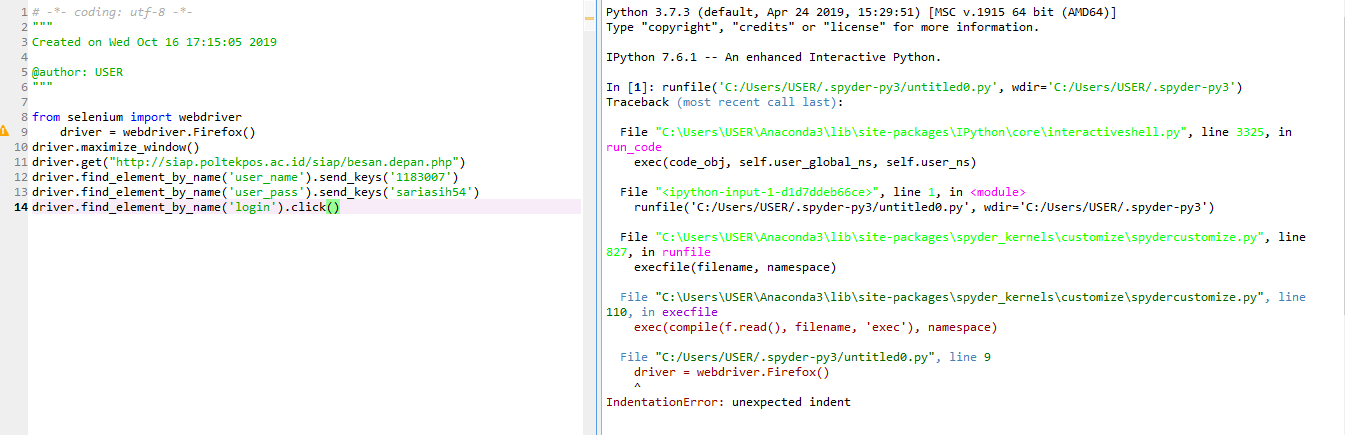
\includegraphics[scale=0.8]{figure/identasi1.png}
\center
\caption{eror identasi}
\end{figure}

\item cara menangani eror
\par
1.Perhatikan Warning kesalahan yang muncul pada jendela iPython Console
terhadap baris tersebut
2.Setelah itu perbaiki kesalahan yang terjadi sehingga tanda warning pada
line tersebut menghilang

\begin{figure}[h]
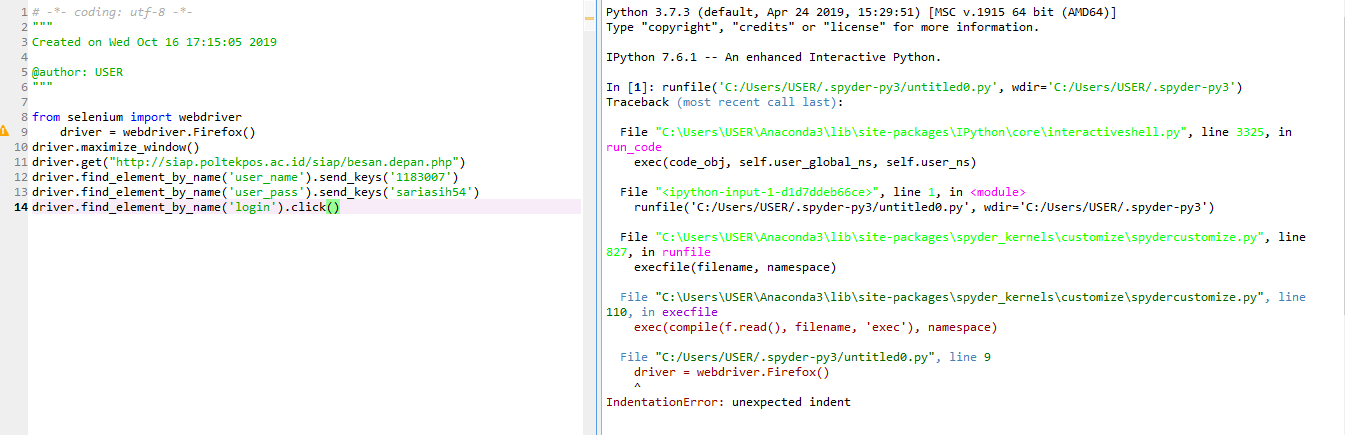
\includegraphics[scale=0.8]{figure/identasi1.png}
\center
\caption{cara menangani eror}
\end{figure}

\begin{figure}[h]
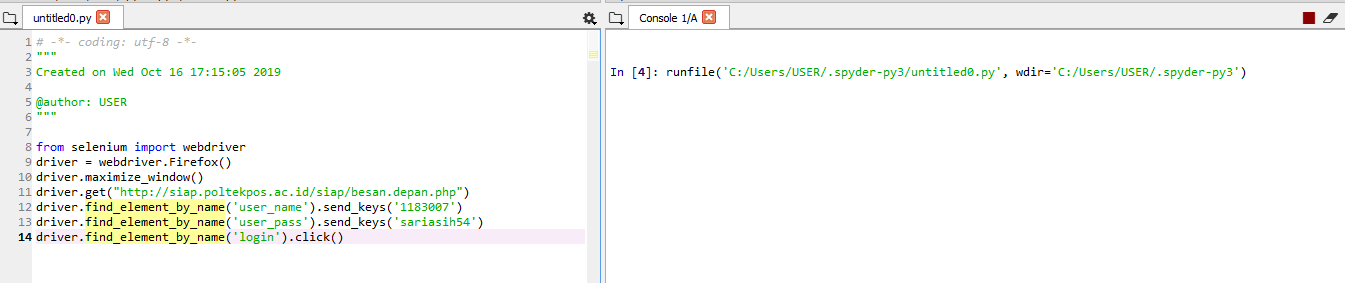
\includegraphics[scale=0.8]{figure/identasi2.png}
\center
\caption{cara menangani eror}
\end{figure}

\end{enumerate}